% **************************************************************************************************************
% A Classic Thesis Style
% An Homage to The Elements of Typographic Style
%
% Copyright (C) 2012 Andr\'e Miede http://www.miede.de
%
% If you like the style then I would appreciate a postcard. My address 
% can be found in the file ClassicThesis.pdf. A collection of the 
% postcards I received so far is available online at 
% http://postcards.miede.de
%
% License:
% This program is free software; you can redistribute it and/or modify
% it under the terms of the GNU General Public License as published by
% the Free Software Foundation; either version 2 of the License, or
% (at your option) any later version.
%
% This program is distributed in the hope that it will be useful,
% but WITHOUT ANY WARRANTY; without even the implied warranty of
% MERCHANTABILITY or FITNESS FOR A PARTICULAR PURPOSE.  See the
% GNU General Public License for more details.
%
% You should have received a copy of the GNU General Public License
% along with this program; see the file COPYING.  If not, write to
% the Free Software Foundation, Inc., 59 Temple Place - Suite 330,
% Boston, MA 02111-1307, USA.
%
% **************************************************************************************************************
% Note:
%    * You must not use "u etc. in strings/commands that will be spaced out (use \"u or real umlauts instead)
%    * New enumeration (small caps): \begin{aenumerate} \end{aenumerate}
%    * For margin notes: \marginpar or \graffito{}
%    * Do not use bold fonts in this style, it is designed around them
%    * Use tables as in the examples
%    * See classicthesis-preamble.sty for useful commands
% **************************************************************************************************************
% To Do:
%		 * [high] Check this out: http://www.golatex.de/koma-script-warnung-in-verbindung-mit-listings-package-t2058.html
%    * [medium] mathbb in section-titles/chapter-titles => disappears somehow in headlines!!!
% **************************************************************************************************************
\documentclass[ twoside,openright,titlepage,numbers=noenddot,headinclude,%1headlines,% letterpaper a4paper
                footinclude=true,cleardoublepage=empty,abstractoff, % <--- obsolete, remove (todo)
                BCOR=5mm,paper=a4,fontsize=11pt,%11pt,a4paper,%
                ngerman,american,%
                ]{scrreprt}

%********************************************************************
% Note: Make all your adjustments in here
%*******************************************************
\input{classicthesis-config}

%********************************************************************
% Hyphenation
%*******************************************************
%\hyphenation{put special hyphenation here}

% ********************************************************************
% GO!GO!GO! MOVE IT!
%*******************************************************
\begin{document}
\frenchspacing
\raggedbottom
\selectlanguage{american} % american ngerman
%\renewcommand*{\bibname}{new name}
%\setbibpreamble{}
\pagenumbering{roman}
\pagestyle{plain}
%********************************************************************
% Frontmatter
%*******************************************************
%*******************************************************
% Titlepage
%*******************************************************
\begin{titlepage}
	% if you want the titlepage to be centered, uncomment and fine-tune the line below (KOMA classes environment)
	\begin{addmargin}[-1cm]{-3cm}
    \begin{center}
        \large
        \includegraphics[width=3cm]{gfx/hft_logo}
        \includegraphics[width=3cm]{gfx/mhm_logo}
         \\ \medskip  

        \hfill

        \vfill

        \begingroup
            \color{Maroon}\spacedallcaps{\myTitle} \\ \bigbreak
        \endgroup
        \mySubtitle
        \vfill 

        \spacedlowsmallcaps{\myName}


        

          
        \myDegree \\
        \bigskip \medskip
        \spacedlowsmallcaps{Supervisors}\\
        \myProf \\
        \myOtherProf \\
        %\myDepartment \\                            
        %\myFaculty \\
        %\myUni \\ 
        \bigskip
        \bigskip
        \spacedlowsmallcaps{Supervising Company} \\
        \textit{MHM Systemhaus GmbH}\\
        \bigskip
        \bigskip
        \spacedlowsmallcaps{Faculty} \\
        Fakultät Vermessung, Mathematik und Informatik\\        
        \bigskip
        \bigskip

        \myTime

        \vfill                      

    \end{center}  
  \end{addmargin}       
\end{titlepage}   
\include{FrontBackmatter/Titleback}
\cleardoublepage%*******************************************************
% Dedication
%*******************************************************
\thispagestyle{empty}
%\phantomsection 
\refstepcounter{dummy}
\pdfbookmark[1]{Dedication}{Dedication}

\vspace*{4cm}

\medskip

\begin{center}
    This thesis, unlike many others, is printed in both sides. This has been done on purpose and is intended to save paper. \\ \bigskip
    \bigskip
    If you didn't receive a hard copy of this work, please \textsc{do not} print it.\\ \bigskip \bigskip
    \includegraphics[width=.45\linewidth]{gfx/gogreen}
\end{center}
\cleardoublepage%*******************************************************
% Declaration
%*******************************************************
\refstepcounter{dummy}
\pdfbookmark[0]{Declaration}{declaration}
\chapter*{Declaration}
\thispagestyle{empty}
I hereby declare that this Final Thesis has been completed independently and without the use of external help, other than the specified sources. Pieces of literature that were taken literally or in spirit out of these sources are marked as such. Furthermore I declare that this work has not been published elsewhere or submitted elsewhere as examination performance.\\
\newline

Hiermit erkläre ich, dass ich die vorliegende Abschlussarbeit selbständig verfasst und  keine anderen als die angegebenen Quellen und Hilfsmittel verwendet habe. Alle Stellen, die wörtlich oder sinngemäß aus den Quellen entnommen wurden, sind als solche kenntlich gemacht. Weiterhin erkläre ich, dass die Arbeit nicht anderweitig veröffentlicht oder an anderer Stelle als Prüfungsleistung vorgelegt wurde.
\bigskip
 
\noindent\textit{\myLocation, \myTime}

\smallskip

\begin{flushright}
    \begin{tabular}{m{5cm}}
        \\ \hline
        \centering\myName \\
    \end{tabular}
\end{flushright}

%\cleardoublepage\include{FrontBackmatter/Foreword}
\cleardoublepage%*******************************************************
% Abstract
%*******************************************************
%\renewcommand{\abstractname}{Abstract}
\pdfbookmark[1]{Abstract}{Abstract}
\begingroup
\let\clearpage\relax
\let\cleardoublepage\relax
\let\cleardoublepage\relax
\vfill
\chapter*{Abstract}
This work is divided into 4 parts that are preceded by an introduction and a glance at the history of \emph{MHM Systemhaus GmbH}, the company that kindly gave me the opportunity to write this paper and develop a mobile application for their eRecruiting Service.

In \spacedlowsmallcaps{Part 1} we will take a brief look into the history of mobile computing itself and of the currently available platforms. We will also discuss some of the distribution and development challenges that a multi-platform application has to face, before being published. 

\spacedlowsmallcaps{Part 2} will focus on the steps it takes to design a mobile application, the possibilities for multi-platform development and the challenges one has to consider when choosing the best approach and framework for cross-platform development. It will also evaluate two of the most popular frameworks based on our requirements and as a result will give us the best framework for us to use in the development of our mobile application.

In \spacedlowsmallcaps{Part 3} we will discuss what the cloud actually is and how we can optimize a service to create a seamless connection to a mobile device. We also will review the challenges one has to consider in order to securely connect an application to a cloud service and the different communication types that are available to us.

Finally, \spacedlowsmallcaps{Part 4} will collect all of the topics previously discussed and will focus on the development of a real world application using a specially designed Rails Server Application that connects to the MHM eRecruiting Systems and acts as cloud service.       


\vfill


\endgroup			

\vfill
%\include{FrontBackmatter/Publication}
\cleardoublepage%*******************************************************
% Acknowledgments
%*******************************************************
\pdfbookmark[1]{Acknowledgments}{acknowledgments}

\begin{flushright}{\slshape    
    We have seen that computer programming is an art, \\ 
    because it applies accumulated knowledge to the world, \\ 
    because it requires skill and ingenuity, and especially \\
    because it produces objects of beauty.} \\ \medskip
    --- \defcitealias{knuth:1974}{Donald E. Knuth}\citetalias{knuth:1974} \citep{knuth:1974}
\end{flushright}



\bigskip

\begingroup
\let\clearpage\relax
\let\cleardoublepage\relax
\let\cleardoublepage\relax
\chapter*{Acknowledgments}
I'd like to thank my family for always supporting me in whatever I wanted to do. I'd also like to thank my lovely girlfriend with all my heart. She has helped me become a better person and helped me strive for bigger goals.


I dedicate this work to my parents, because without their help I wouldn't be where I am today.
\bigskip

\textit{Agradezco a mi familia por toda su ayuda y apoyo y por darme la confianza para siempre perseguir mis metas. También a mi novia, quien me ha ayudado a ser una mejor persona y me empuja a perseguir mejores metas.}

\textit{Este trabajo se lo dedico a mis padres, porque sin su ayuda, no estaría donde estoy ahora. ¡Gracias por todo su amor y dedicación!}

\endgroup




\pagestyle{scrheadings}
\cleardoublepage%*******************************************************
% Table of Contents
%*******************************************************
%\phantomsection
\refstepcounter{dummy}
\pdfbookmark[1]{\contentsname}{tableofcontents}
\setcounter{tocdepth}{2} % <-- 2 includes up to subsections in the ToC
\setcounter{secnumdepth}{3} % <-- 3 numbers up to subsubsections
\manualmark
\markboth{\spacedlowsmallcaps{\contentsname}}{\spacedlowsmallcaps{\contentsname}}
\tableofcontents 
\automark[section]{chapter}
\renewcommand{\chaptermark}[1]{\markboth{\spacedlowsmallcaps{#1}}{\spacedlowsmallcaps{#1}}}
\renewcommand{\sectionmark}[1]{\markright{\thesection\enspace\spacedlowsmallcaps{#1}}}
%*******************************************************
% List of Figures and of the Tables
%*******************************************************
\clearpage

\begingroup 
    \let\clearpage\relax
    \let\cleardoublepage\relax
    \let\cleardoublepage\relax
    %*******************************************************
    % List of Figures
    %*******************************************************    
    %\phantomsection 
    \refstepcounter{dummy}
    %\addcontentsline{toc}{chapter}{\listfigurename}
    \pdfbookmark[1]{\listfigurename}{lof}
    \listoffigures

    \vspace*{8ex}

    %*******************************************************
    % List of Tables
    %*******************************************************
    %\phantomsection 
    \refstepcounter{dummy}
    %\addcontentsline{toc}{chapter}{\listtablename}
    \pdfbookmark[1]{\listtablename}{lot}
    \listoftables
        
    \vspace*{8ex}
    \newpage
    
    %*******************************************************
    % List of Listings
    %*******************************************************      
	  %\phantomsection 
    \refstepcounter{dummy}
    %\addcontentsline{toc}{chapter}{\lstlistlistingname}
    \pdfbookmark[1]{\lstlistlistingname}{lol}
    \lstlistoflistings 

    \vspace*{8ex}
       
    %*******************************************************
    % Acronyms
    %*******************************************************
    %\phantomsection 
    \refstepcounter{dummy}
    \pdfbookmark[1]{Acronyms}{acronyms}
    \markboth{\spacedlowsmallcaps{Acronyms}}{\spacedlowsmallcaps{Acronyms}}
    \chapter*{Acronyms}
    \begin{acronym}[UML]
        \acro{AOT}{Ahead Of Time}
        \acro{API}{Application Programming Interface}
        \acro{CI}{Continuous Integration}
        \acro{DRY}{Don't Repeat Yourself}
        \acro{IaaS}{Infrastructure as a Service}
        \acro{IDE}{Integrated Development Environment}
        \acro{IL}{Intermediate Language}
        \acro{IP}{Internet Protocol}
        \acro{JIT}{Just In Time}
        \acro{JPA}{Job Portal Aggregator}
        \acro{JSON}{JavaScript Object Notation}
        \acro{LINQ}{Language-Integrated Query}
        \acro{MVC}{Model-View-Controller}
        \acro{MVVM}{Model-View-ViewModel}
        \acro{NIST}{National Institute of Standards and Technology}
        \acro{OEM}{Original Equipment Manufacturer}
        \acro{ORM}{Object-Relational Mapping}
        \acro{OS}{Operating System}
        \acro{PaaS}{Platform as a Service}
        \acro{PDA}{Personal Digital Assistant}
        \acro{SaaS}{Software as a Service}
        \acro{SDK}{Software Development Kit}
        \acro{SOAP}{Simple Object Access Protocol}
        \acro{REST}{REpresentational State Transfer}
        \acro{TDD}{Test Driven Development}       
        \acro{UI}{User Interface}
        \acro{UML}{Unified Modeling Language}
        \acro{URI}{Uniform Resource Identifier}
        \acro{VM}{Virtual Machine}
        \acro{XML}{eXtensible Markup Language}
    \end{acronym}                     
\endgroup

\cleardoublepage
%********************************************************************
% Mainmatter
%*******************************************************
\pagenumbering{arabic}
%\setcounter{page}{90}
% use \cleardoublepage here to avoid problems with pdfbookmark
\cleardoublepage
%************************************************
\chapter{Introduction}\label{ch:introduction}
%************************************************
The arena of mobile computing has changed dramatically in the past 10 years. It has advanced very rapidly, leaving behind those who couldn't keep up with the development pace and taking the innovators and visionaries for the ride of their lives.

Mobile Computing is not only changing the way we do business, but also the way we live and interact with our environment. It has become so common to always have a computing device with us, that the demand for useful applications has skyrocketed, thus making the development of software for these devices a very lucrative field.

But, even though the devices in our pockets get more powerful year by year, very few applications rely solely on the data and computing power inside the device. The most useful applications are always connected to a magical place called \spacedlowsmallcaps{the cloud}.

But what exactly is The Cloud? In this work we will learn all about the different types of services that can run on top a cloud infrastructure and how we can communicate with these services.

And, where do mobile applications come into play? They are actually very important. The advancement in mobile technology has fueled an entire economic growth for mobile software development. Every big company out there wants to have a presence inside mobile devices, just like when the internet was booming and they wanted to have a web presence.

All this demand for mobile software solutions has been the catalyst in the development of different frameworks that can help developers create applications compatible with the different Mobile Operating Systems out there.

This particular conundrum is the main focus of this work. We will investigate and evaluate the most popular frameworks available and after we make a decision, we will get our hands dirty and dive into the creation of a multi-platform mobile application for Android and iOS, but not before we talk about the history of mobile computing and discuss the different mobile platforms currently available.

\section{Goals of this Work}

This is work part of my Bachelor's Thesis and is required for me to graduate from the University of Applied Sciences in Stuttgart, Germany and was produced in conjunction with \textit{MHM Systemhaus GmbH}. The second part is an oral presentation regarding what's being discussed here, plus a demonstration of the application that resulted from this endeavor.

The commercial goals of this work, as discussed with \textit{MHM} are:
\begin{itemize}
\item Create a multi-platform application that aggregates open job positions from different companies into a single view.
\item The application must be generic, meaning all clients of \textit{MHM} should show up and there should be a way to see only the open positions of one client.
\item There should be search functionality and past searches should be saved.
\item Notifications should be sent based on past searches.
\item Implementation of a so-called "Upload-Application", so that the user can apply to a job, directly from the app, by uploading his files.
\end{itemize}

The academic goals of this work are:
\begin{itemize}
\item Investigate how The Cloud works and understand its impact on our field of work and on society.
\item Learn about the different alternatives for the creation of a multi-platform mobile application
\item Deepen my knowledge about mobile technologies and mobile application development.
\item Learn a new Programming Language and a new way of creating mobile applications.
\end{itemize}


\section{Writing Conventions}
Newly introduced concepts that are relevant to a chapter will be described there, for all other concepts, please refer to the Glossary inside \autoref{glos}.

\spacedlowsmallcaps{Important Note:} Some things of the style used for this work might look unusual at first glance, many people feel so in the beginning.
However, all things were intentionally designed to be as they are.










   


%************************************************
\chapter{MHM-Systemhaus GmbH}\label{ch:mhm}
%************************************************

\section{History}
MHM-Systemhaus GmbH (MHM) is a German IT Company based in Stuttgart that was founded on April \nth{1}, 2001, by Armin Mendle, Christian Hasenstab and Steffen Michel. Currently, only Mendle and Michel manage the firm, due to Hasenstab's departure in 2005 as the company switched from a GbR to a GmbH\marginpar{GbR \& GmbH are types of legal entities in Germany.}

MHM develops customized Talent Management Software, eRecruiting Applications and ERA-Software\footnote{EntgeltRahmenAbkommen is a regulated compensation agreement in the Metal \& Electronic Industry}. These solutions are developed as Web Applications and are adaptable to existing HR-Processes\marginpar{HR: Human Resources}.

Two of the biggest advantages of the MHM Software Solutions are the priority it gives to data protection and the high adjustability to processes that the clients already have in place. Because of this, MHM was audited in 2010 and certified to comply with German Data Protection Law (\textsection{11} BDSG).\cite{michel:2012}

Until 2011, development of the MHM eRecruiting applications was done using an  Java Framework developed in-house that is still maintained for older clients, but no longer updated. Since then, the team has moved the entire eRecruiting System to Ruby on Rails, an object oriented, web development framework based on the \ac{MVC} architecture pattern.\footnote{\url{http://rubyonrails.org}} The new framework gives the development team a high amount of flexibility when customizing the application and provides a level of abstraction that assures a faster learning curve for new developers. The reason for this complete rewrite was to have an application that is future-proof, capable of being maintained and upgraded for years to come.

\section{MHM eRecruiting}
The Centre of Human Resources Information Systems of the University of Bamberg and Frankfurt am Main in conjunction with Monster Worldwide Deutschland GmbH surveyed 1000 small- and medium-sized Companies in Germany about their Recruiting procedures in 2012.\cite[p. 6]{weitzel:2012}

The study showed that 37.5\% of all new recruits came from job postings either listed on the company's website or from Online Job Markets. The percentage of paper-based Applications has diminished constantly for the past few years and 2012 was the first year that companies preferred applications via E-Mail. Some companies even predict that by the year 2016 less than a third of all applications will be paper based. Social Media plays a huge roll in this change. 48.3\% of the surveyed companies see the possibility of reaching more candidates by using Facebook, LinkedIn or XING.\cite[p. 8]{weitzel:2012}

The MHM eRecruiting Application can be used for paper-based applications as well as online applications. It offers the possibility to publish any vacant position to a number of different channels. It can be automatically posted on Facebook or XING, or on external Job Portals like Stepstone and also on the customer's web site.

This level of automation and practicality is what has made the eRecruiting solution so successful. We want to continue offering more options to customers, which is why the main goal of this thesis is to develop a Mobile Application that acts as another Job Portal Channel and aggregates vacant positions, from customers that wish to use the feature, into an easy to use, always available, always online, mobile platform. %thus giving more exposure to each vacancy and 


















 
   

\ctparttext{
{\slshape
Today, most people approach mobile computing the way they did the Web 15 years ago. I have some business process or operations. Here's this new channel, the Internet. How do I take what I'm doing now and put it on the Web?

We know how that worked out for most companies -- not so well. Entire industries and operations were transformed by the Web, just not in ways that people initially imagined. But human nature being what it is, this is exactly the approach people are taking again with mobile.

It's not until we take a step back and say, let's just forget the old business processes and consider what's new and innovative about this new technology. Then we can get a true picture of the future of mobility.\\\bigskip
}

--- \defcitealias{bloom:2012}{Paul Bloom}\citetalias{bloom:2012} \citep{bloom:2012}
}

\part{The world of mobile}
%*****************************************
\chapter{Short History of mobile computing}\label{ch:history}
%*****************************************

How you define mobile computing plays a huge role in its history, because depending on the definition, it can begin as early as 1971 or as late 1984.

\begin{quotation}
Mobile computing is human-computer interaction by which a computer is expected to be transported during normal usage.\footnote{\url{http://en.wikipedia.org/wiki/Mobile_computing}}
\end{quotation}

If you go with 1971 as the beginning of mobile computing, you come across a very simple, though very advanced for the time, calculator. The Busicom LE-120A 'Handy-LE' was the first true pocket sized calculator. Impressive as it may be for the time, a calculator is not something many people would consider as proper computing.

In 1981 the Osborne 1 portable computer came to the market. It was the very first computer designed for users to pack up and carry. The Osborne 1 offered a 5-inch diagonal screen, two full size floppy drives, a keyboard that snapped onto the system, and a handle in the back for easy carrying. But, at 11 kg in weight, it is difficult to consider it as truly portable.\footnote{\url{http://oldcomputers.net/osborne-1.html}}

In 1982 the GRiD Compass 1101 was released. Considered by many to be the grandfather of current laptops, the Compass 1101 was the first portable computer to include the now ubiquitous clamshell design that all modern laptops have, and weighing in at only 4.5 kg, it was the first truly portable computer.\footnote{\url{http://oldcomputers.net/grid1101.html}}

Here is where the story we find interesting begins, but since this thesis caters for a different type of portable computing device, we need to fast forward a little bit in time to 1991 to encounter the first pocket computer, the Psion Series 3.

Since 1982, portable computing devices have become smaller and smarter and in 1991 Psion released the first palmtop minicomputer, a personal organizer that featured a word processor, a spreadsheet, a contacts database, a sketch program, a calculator and a clock.\footnote{\url{http://www.computerworlduk.com/slideshow/mobile-wireless/3267504/}}

But Psion wasn't alone for long. In 1992 Apple Computer released their \ac{PDA} Device called the Newton, but the popularity of these devices was eclipsed when Palm released the Palm Pilot 1000 in 1996. Like every other \ac{PDA} the Pilot let you keep a to do list, a calendar, a contacts database and short memos all in a small, stylus input-based handheld device, but Palm's Graffiti handwriting recognition technology did better job at accepting stylus input than Newton and earlier handwriting systems did, thus becoming more popular than its competitiors.\footnote{\url{http://www.computerworlduk.com/slideshow/mobile-wireless/3267504/}}

After 1996 many different manufactures entered the \ac{PDA} market, and Palm continued to innovate on its line of devices, but in 2002 a cellular phone company called Research in Motion came up with the BlackBerry 5810, a \ac{PDA} that featured phone and email functionality. This device popularized several technologies that users value in smartphones today, such as push email and end-to-end data encryption.\footnote{See above}

Innovations kept being made every year, with different devices coming to market and combining phones with \ac{PDA}s. The first smartphones came around the same time and they too started incorporating more and more features.

By 2007 smartphones were almost omnipresent in the enterprise world, but they were still too expensive and not user friendly enough for the mass market. That is until Apple released the first iPhone, with its intuitive interface and powerful computing ability, it changed the way smartphones were made, removing physical keyboards and making the entire experience as easy and pleasant as possible.
 

  

%Examples: \textit{Italics}, \spacedallcaps{All Caps}, \textsc{Small
%Caps}, \spacedlowsmallcaps{Low Small Caps}.

\enlargethispage{2cm}
\begin{figure}[bth]
        \myfloatalign
        \subfloat[Osborne 1]
        {\includegraphics[width=.45\linewidth]{gfx/osborne}} \quad
        \subfloat[GRiD Compass 1101]
        {\label{fig:example-b}%
         \includegraphics[width=.45\linewidth]{gfx/compass}} \\
        \subfloat[Palm Pilot 1000]
        {\includegraphics[width=.45\linewidth]{gfx/palm}} \quad
        \subfloat[BlackBerry 5810]
        {\includegraphics[width=.45\linewidth]{gfx/blackberry}}
        \caption[First mobile computing devices]{First mobile computing devices}\label{fig:example}
\end{figure}
%************************************************
\chapter{Current mobile Platforms}\label{ch:m_plats} % $\mathbb{ZNR}$
%************************************************
\section{Android}
\spacedlowsmallcaps{Android} is a Linux based operating system specially designed for touchscreen devices like smartphones or tablets. It began as the brain-child of a new company called Android, Inc. back in 2003.

\begin{quotation}
Android, Inc. was founded in Palo Alto, California in October 2003 by Andy Rubin (co-founder of Danger), Rich Miner (co-founder of Wildfire Communications, Inc.), Nick Sears (once VP at T-Mobile), and Chris White (headed design and interface development at WebTV) to develop, in Rubin's words "smarter mobile devices that are more aware of its owner's location and preferences". The early intentions of the company were to develop an advanced operating system for digital cameras, when it was realised that the market for the devices was not large enough, and diverted their efforts to producing a smartphone operating system to rival those of Symbian and Windows Mobile (Apple's iPhone had not been released at the time). Despite the past accomplishments of the founders and early employees, Android Inc. operated secretly, revealing only that it was working on software for mobile phones. That same year, Rubin ran out of money. Steve Perlman, a close friend of Rubin, brought him \$10,000 in cash in an envelope and refused a stake in the company.
\cite{wikipedia:android}
\end{quotation}

Google bought Android, Inc. in 2005 and made it a wholly owned subsidiary. The most important employees stayed and started working on what later would become the Android Operating System.

Up until the release of the first Android Device on October \nth{22}, 2008, Google conducted secret meetings with many handset and chip manufacturers to discuss the creation of a new consortium, the Open Handset Alliance, with the goal to develop open standards for mobile devices. The Alliance was unveiled on November \nth{5}, 2007.\footnote{\url{http://www.openhandsetalliance.com/press_110507.html}}


After the first device with Android, the HTC Dream, was released there has been a major surge of devices using Android. Hardware manufacturers from all over the world have chosen Android as their favourite operating system, not only for smartphones and tablets but also for embedded devices like the Cotton Candy Stick from FXI Technologies and even gaming consoles like the Ouya. %They have gone the Android route to give their devices a robust and secure operating system.


The development of system features and other components has been done at a steady pace, releasing new versions of the OS every couple of months. The team has chosen to give colourful names to each release, always in alphabetical order and always named after a dessert or a sweet treat. A closer look at \autoref{fig:android1} and \autoref{fig:android2} should give you  better overview over the different versions of Android and what each new version brought forth.   

\begin{figure}
    \hbox{
        \hspace{-4em}
        {\includegraphics[width=1.5\linewidth]{gfx/android-history1}}
        \caption[Visual History of Android, Part 1]{Visual History of Android}\label{fig:android1}
    }
\end{figure}
\begin{figure}
    \hbox{
        \hspace{-12em}
        {\includegraphics[width=1.55\linewidth]{gfx/android-history2}}
        \caption[Visual History of Android, Part 2]{Visual History of Android\footnotemark}\label{fig:android2}
    }
\end{figure}
\footnotetext{Source: \url{http://visual.ly/sweet-history-android}}\\

\subsection{The Android Open Source Project}
One of the best features and assets of Android is that it is 100\% Open Source. This allows everyone with the necessary knowledge to contribute to the development of the platform and also to modify it in every way you want.


This is exactly what the guys behind CyanogenMod have done. They took the regular Android Operating System and added many features and improvements to the core experience, making it the most popular unofficial Android OS.


But these types of modifications are not only common inside hobbyist communities, big corporations also contribute code to the Android Project. Some even modify the code so much, that it becomes almost unrecognisable. That is exactly what Amazon did. They took the Android OS and heavily modified it in order to install it in their Kindle Fire family of tablets.


Using an Open Source Model also guarantees Android an independent future from Google. Even if Google stops supporting \marginpar{Note: Google is unlikely to stop supporting Android} Android, the community will pick up the pieces and continue with its development and will guarantee its longevity.
 
\section{BlackBerry}
\section{iOS}
\begin{figure}[H]
    \begin{center}
        {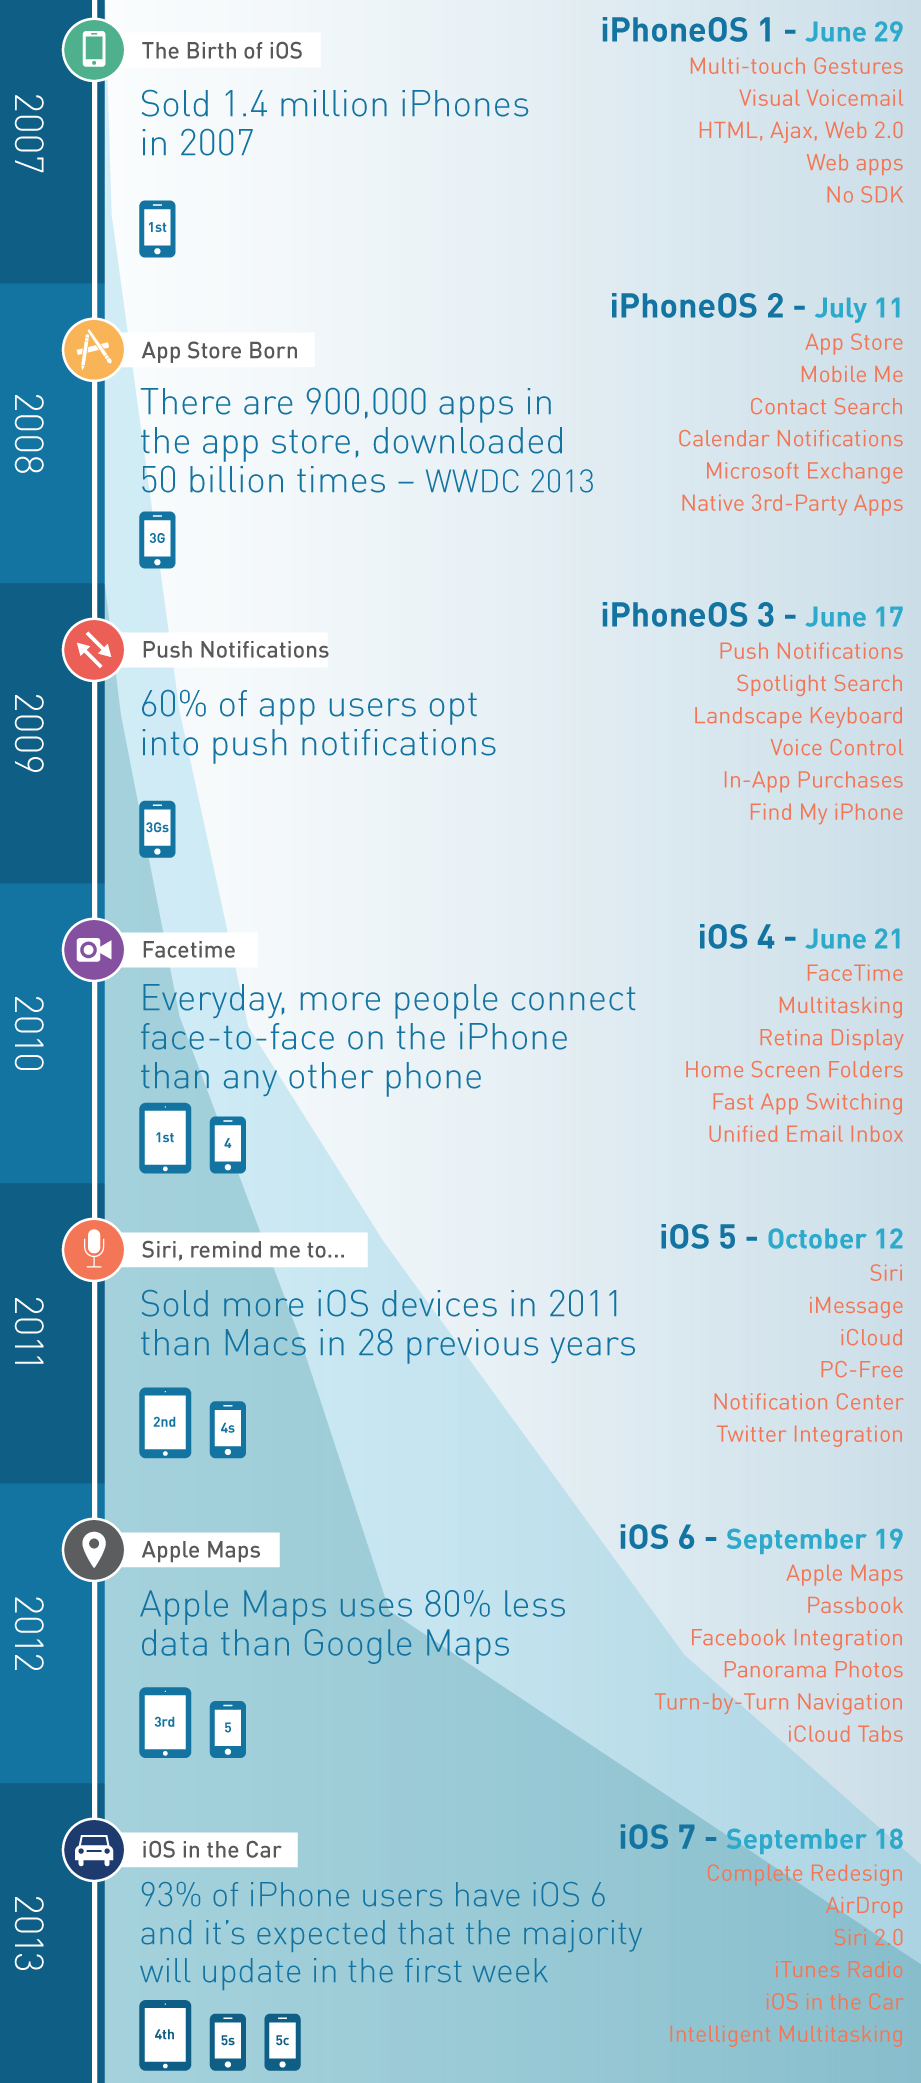
\includegraphics[width=.90\linewidth]{gfx/ios-history}}
        \caption[Visual History of iOS]{Visual History of iOS\footnotemark}\label{fig:ios}
    \end{center}
\end{figure}
\footnotetext{Source: \url{http://visual.ly/history-ios}}\\

\section{Windows Phone}
\section{Other platforms worth noting}
The platforms mentioned above are the most popular ones. Together they control around 95\% of the mobile market, however, there are companies like Mozilla and Cononical that want to enter the competition and bring forth completely new ideas on what a mobile operating system should be.

\subsection{Firefox OS}
\spacedlowsmallcaps{Firefox OS} is Mozilla's entry to the mobile market. It hopes to revolutionise the mobile ecosystem by proposing that all applications for the device be programmed using Web Technologies.

\begin{quotation}
On July 25, 2011, Dr. Andreas Gal, Director of Research at Mozilla Corporation, announced the "Boot to Gecko" Project (B2G) on the mozilla.dev.platform mailing list. The project proposal was to "pursue the goal of building a complete, standalone operating system for the open web" in order to "find the gaps that keep web developers from being able to build apps that are – in every way – the equals of native apps built for the iPhone [iOS], Android, and WP7 [Windows Phone 7]." The announcement identified these work areas: new web APIs to expose device and OS capabilities such as telephone and camera, a privilege model to safely expose these to web pages, applications to prove these capabilities, and low-level code to boot on an Android-compatible device.
This led to much blog coverage. According to Ars Technica, "Mozilla says that B2G is motivated by a desire to demonstrate that the standards-based open Web has the potential to be a competitive alternative to the existing single-vendor application development stacks offered by the dominant mobile operating systems."
\cite{wikipedia:firefox}
\end{quotation}

In 2012 B2G was rebranded as Firefox OS in honour of the company's flagship product, the Firefox Web Browser.


Some preview units have been shipped to journalists and developers, in order to gain some traction, but the system has not come to production, yet. 

\begin{quotation}
In February 2013, Mozilla announced plans for global commercial roll-out of Firefox OS. Mozilla announced at a press conference before the start of Mobile World Congress in Barcelona that the first wave of Firefox OS devices will be available to consumers in Brazil, Colombia, Hungary, Mexico, Montenegro, Poland, Serbia, Spain and Venezuela. Firefox have also announced that LG Electronics, ZTE, Huawei and TCL Corporation have committed to making Firefox OS devices.
\cite{wikipedia:firefox}
\end{quotation}

 

\subsection{Ubuntu Phone}
\spacedlowsmallcaps{Ubuntu Phone} is Conical's horse in the mobile race. With it, Canonical hopes to disturb the mobile market by offering a single operating system capable of being a Mobile OS and a Desktop OS. As Canonical's own website puts it, 

\begin{quotation}
High-end smartphones have a brain as powerful as ultra-light laptops. Ubuntu uniquely enables a new category of convergence device – phones that dock to become full PCs and thin clients; enabling enterprise IT departments to replace phones, thin clients and laptops with a single secure corporate device.\\

Operators targeting the enterprise market with LTE can now deliver a full laptop/phone solution, with Windows apps delivered over LTE from the corporate data center. And operators in emerging markets can deliver desktop applications to the converged device over LTE as a premium data service.\footnote{\url{http://www.ubuntu.com/phone/operators-and-oems}}
\end{quotation}


\spacedlowsmallcaps{Ubuntu Phone} is still in the early stages of development, but has already gained the backing of major OEM's and carriers around the world. Once it hits the market, it will become the next player to watch, doubtlessly bringing new ideas and features to the table.  
















 
\cleardoublepage
\ctparttext{Part 2 Text}
\part{Developing multi-platform applications}
%************************************************Ready v1
\chapter{Frameworks for multi-platform development}\label{ch:frameworks}
%************************************************
There are numerous frameworks that have been developed over the years to facilitate the creation of multi-platform applications. Just like in the 90s, when vendors saw market opportunities in releasing multi-platform applications for the desktop, most of the solutions available for cross-platform mobile development are of the commercial nature.


However, \marginpar{PhoneGap is the commercial name of the Apache Cordova Open Source Project.} some open source players do exist. They have been gaining popularity and better features over time, some have even been backed by bigger organisations, and now offer both free and commercial packages. Examples worth noting in this category are PhoneGap, backed by Adobe and MonoTouch, backed by Xamarin.
\graffito{MonoTouch is an open source implementation of Microsoft's .NET Framework.}

\section{Types of Frameworks}
When it comes to choosing the adequate framework to use for the development of your application, there are many options that vary in number of features, pricing and support; but they can all be sorted into three distinct categories, based on the type of application they produce at the end. These categories are:
\begin{enumerate}
    \item HTML5 Web Applications (\autoref{sec:web_app})
    \item Hybrid Applications (\autoref{sec:hyb_app})
    \item Pseudo-Native Applications (\autoref{sec:pseudo_app})
\end{enumerate}

You should always keep in mind the advantages and drawbacks of each when choosing which type of framework is the best for your needs, but let us take a look at \autoref{tab:frameworks} first. It should give you an overview over the technologies used and the type of applications produced by the most popular cross-platform frameworks. We will discuss each type in detail later on.\newline

\begin{table}[H]
    \myfloatalign
  \begin{tabularx}{\textwidth}{Xll} \toprule
    \tableheadline{Name} & \tableheadline{Language} & \tableheadline{Type}\\ 
    \midrule
    Web frameworks & HTML \& Javascript & Web App\\
    Corona SDK & Lua & Pseudo-Native\\
    Embarcadero & Delphi \& C++ & Pseudo-Native\\
    Icenium\textsuperscript{*} & Javascript & Hybrid\\
    Intel XDK\textsuperscript{*} & Javascript & Hybrid\\
    PhoneGap\textsuperscript{*} & Javascript & Hybrid\\
    Rhodes & Ruby \& Javascript & Hybrid\\
    Titanium SDK & Javascript & Hybrid \& Pseudo-Native\\
    Xamarin & C\# + Native UI & Pseudo-Native\\      
    %\midrule
    \bottomrule
  \end{tabularx}
  \caption[Characteristics of the most popular cross-platform frameworks]{Overview of some characteristics of the most popular cross-platform frameworks\footnotemark}  \label{tab:frameworks}
\end{table}
\marginpar{\vbox{\vspace{-24em}\textsuperscript{*} All of these frameworks are based on Apache Cordova}}
\footnotetext{Information taken from the Framework's respective website}  

As \autoref{tab:frameworks} lets us see, the majority of available frameworks seem to be those that deliver a hybrid application. This phenomenon can be explained by what \citeauthor{allen:2010} express in their book about Cross-Platform Development:
\begin{quotation}
These new smartphone frameworks are influenced by the rapid application development techniques we are seeing in web development today. There are three specific techniques in web application development that are borrowed for these non-web frameworks: 1) layout with mark-up (HTML/CSS); 2) using URLs to identify screen layouts and visual state; and 3) incorporating dynamic languages, such as Javascript and Ruby.

A generation of designers and user interface developers are fluent in HTML and CSS for layout and construction of visual elements. Additionally, addressing each screen by a unique name in a sensible hierarchy (URL) with a systemized way of defining connections between them (links and form posts) has created a lingua franca understood by visual and interactions designers, information architects, and programmers alike. This common language and its standard implementation patterns led to the development of frameworks and libraries that significantly speed application development on the Web. These patterns are now being applied to the development of mobile applications as common techniques by individual developers as well as in cross-platform frameworks.
\cite[p. 23]{allen:2010}
\end{quotation}
Before we dive into each type of framework, \autoref{fig:hybrid_native} should give you a better overview over their capabilities.\\

\marginpar{\autoref{fig:hybrid_native}: The 'Native' label also applies to Pseudo-Native}
\begin{figure}[H]
    \begin{center}
        {\includegraphics[width=1\linewidth]{gfx/Native_html5_hybrid}}
        \caption[Overview of app capabilities. Native vs. Hybrid vs. HTML5]{Overview of app capabilities. Native vs. Hybrid vs. HTML5\footnotemark}\label{fig:hybrid_native}
    \end{center}
\end{figure}
\footnotetext{Source: \url{http://wiki.developerforce.com/page/Native,_HTML5,_or_Hybrid:_Understanding_Your_Mobile_Application_Development_Options}}\\

\subsection{HTML5 Web Applications}\label{sec:web_app}
Just as any other website, \spacedlowsmallcaps{HTML5 Web Applications} can be developed in any language that can be translated to HTML code on runtime. Some examples of these languages are \emph{Ruby, PHP, Python, JSP} or just plain HTML. Some of the most popular web development frameworks, like Ruby on Rails or Synfony\marginpar{Synfony is an MVC Framework for PHP, similar, but not quite as powerful as Rails.}, are very well suited for the development of Web Applications for Mobile Devices.


But having HTML code is not everything, you still need to make it look good in the smaller screen of cellphones and tablets. That's where CSS3 comes into play. With CSS3 you define the look and feel of the application, but you need to define specific rules for devices with a smaller resolution. This can be accomplished in two ways:
\begin{enumerate}
    \item Responsive CSS3 Design
    \item Separate Domain and CSS files for mobile devices
\end{enumerate}
\spacedlowsmallcaps{Responsive CSS3 Design} means you need to distinguish between the different screen sizes and define different rules and properties for each inside your CSS files. With responsive design, changes in screen orientation can also be translated to a different layout, e.g. changing the width of tables or the arrangement of images.


With \spacedlowsmallcaps{Separate Files} you will have to redirect visitors using a mobile device to a different domain and have that domain serve the corresponding CSS files. This approach has some caveats, the most obvious one being the overhead of a different domain with separate HTML and CSS files to maintain and the fact that if you want your layout to react to screen dimension changes, you will most likely need to implement some sort of responsive design, anyway.   
 

These frameworks, however, cannot run inside the mobile device; they need to run on a server, which means that the only way to access the application is through a web browser.


This line of action is best suited for smaller projects that want to present their website or web application in a better way to mobile users, but don't have the resources to hire a full time application developer. They can use the designer they have at hand and just optimise their online presence for portable devices.

\subsection{Hybrid Applications}\label{sec:hyb_app}
\begin{quotation}
Before any cross-platform frameworks existed, many developers found that embedding a Web \ac{UI} in a native application was a practical way to develop mobile applications quickly and make cross-platform applications easier to maintain. The user interface for mobile applications tends to be presented as a series of screens. From a high level, the mobile \ac{UI} can be thought of as having the same flow-of-control as a traditional web site or web application. \cite[p. 28]{allen:2010}
\end{quotation}

\spacedlowsmallcaps{Hybrid Applications} are, in a lot aspects, very similar to HTML5 Web Applications. Both rely on HTML, Javascript and CSS for the definition of the \ac{UI}, but the edge of Hybrid Applications lies in the way they are packaged.

With Hybrid Applications the HTML, et al. are contained within a native package, that allows the framework's \ac{API} to communicate with the operating system, thus leveraging some of the native features the hardware has to offer, e.g. access to the camera, the accelerometer, the GPS, local storage, etc. Access to these features is accomplished via a wrapper that is programmed in each platform's native language and exposes specific methods to an \ac{API} that is accessible from the HTML side using Javascript methods.

By having access to these features, Hybrid Applications can behave like native applications and, since they are contained within a native package, there is no need for the user to open a web browser. It also gives you the advantage of distributing your application via the platform's store.

This approach gives you many added benefits over a normal HTML5 Application, with just some trade-offs. There is a learning curve when dealing with the programming frameworks, but the design and layout are still done in HTML and CSS. One of the main benefits you get is that you now have the possibility to make your application available offline and of course the access to system features like push notifications and background services. 

The downside is that every piece of the \ac{UI} \textsc{needs} to be done in CSS and HTML. There are no native controls, so your application will not look exactly as a native application. 

This approach is best suited for projects that want to offer more functionality with their mobile applications and are willing to invest some time in learning the new framework.  

\subsection{Pseudo-Native Applications}\label{sec:pseudo_app}
\spacedlowsmallcaps{Pseudo-Native Applications} are completely different from the other two types. They do not rely on HTML for the \ac{UI} or on Javascript for communication with native features. These applications are compiled to native code and appear to the device as being truly native.


The way the \ac{UI} is programmed varies between the different frameworks. It can be done using the native tools of each platform; using a visual designer provided by the framework or programatically, using the libraries provided.

Independently from which method is used for the \ac{UI}, the business logic is always done separately in an effort to abstract as much code as possible, that way you don't need to repeat yourself that much.


One of the downsides of taking this approach, is that you have to program the \ac{UI} separately for each platform, which translates into more work and somewhat less maintainability. The advantages, however, can offset all the extra effort.


Let's take a look at the advantages offered by this type of applications:

\begin{description}

\item[Speed:] By not using any interpreted languages, code performance is increased. This is crucial for applications that need to do a lot of calculations quickly or that rely on the assessment of large amounts of data.

\item[Flexibility:] Since the \ac{UI} code is not shared between platforms, it gives you the flexibility to adapt and modify the layout of your application depending on which device is running it. It also gives your application a truly native look \& feel and not an emulated one.

\item[Extra Features:] There are some device features that are not available via Wrapper \ac{API}s but can be accessed by these frameworks, either by extra libraries or by manually extending the framework with native code. This gives you complete control over what you application is capable of doing.
 
\item[Code Reusability:] If you have external libraries that you would like to include in your project, but don't want to rewrite them, using one of these frameworks allows you to include your own libraries in your application if they are programmed in C or C++. 

\end{description}

Using this approach is by no means easy and requires a lot of time and resources, which most often translates into money. But if you want to have complete control over your project, have code that you want to reuse or you simply need your application to run at full speed, this is the right line of action for you.
%************************************************
\chapter{Evaluation of possible frameworks}\label{ch:evaluation}
%************************************************
%\addtocontents{toc}{\protect\clearpage} % <--- just debug stuff, ignore

\ctparttext{Part 3 Text}
\part{The Cloud}
%************************************************
\chapter{The Infrastructure of the Cloud}\label{ch:infrastructure}
%************************************************
%************************************************
\chapter{Connecting to a Cloud Service}\label{ch:conn_cloud}
%************************************************

There are multiple ways of connecting to the different types of cloud services. They vary greatly depending on wich type you want to address. Since we only need to connect to a \ac{SaaS} based service, we will only discuss the possible connection alternatives for it.

A mobile application, like the Job Portal Aggregator, will live inside a device with almost uninterrupted access to the internet. This level of connectivity allows us to consider an abundance of protocols and methods for connecting any type of application to a cloud service.

The whole point of the cloud is to have an infrastructure that is always available and always connected, this means that the main point of entry to these kind of services is the internet, and by default the \ac{IP}. This means that we can use any type of transport layer that builds upon the \ac{IP} Protocol to transmit information from and to a cloud service.\footnote{\url{http://en.wikipedia.org/wiki/IP_protocol}}  

Since the Job Portal Aggregator will be connecting to a \ac{SaaS} Application and, given the fact that the majority of \ac{SaaS} applications are web-based; which means they can be controlled via a web interface or via the HTTP Protocol \cite{mcwherter:2012}; we can consider the following two very different approaches for communicating with our cloud service: \textit{WebSockets} and \textit{RESTful APIs}

\section{RESTful APIs}
In his doctoral dissertation, Roy \citeauthor{fielding:2000} generalized the Web's architectural principles and presented them as an architectural style. He described the interplay between resources, and the role of unique identifiers in such systems. He also talked about using a limited set of operations with strictly defined semantics to build a global infrastructure that can support any type of application. Fielding referred to this architectural style as \ac{REST}. \ac{REST} describes the Web as a distributed hypermedia application whose linked resources communicate by exchanging representations of resource state. \cite{webber:2010}

\begin{quotation}
In a hypermedia system, application states are communicated through representations of uniquely identifiable resources. The identifiers of the states to which the application can transition are embedded in the representation of the current state in the form of links.
\cite[p. 13]{webber:2010}
\end{quotation}

The term RESTful \ac{API} is given to an Application Programming Interface that is accessible via the HTTP Protocol and complies with the \ac{REST} architectural pattern.

One of the biggest advantages of a RESTful \ac{API} is that it allows you to perform different actions based on the state of the application, thus providing constraints on what the user of the application is allowed to do.

Communication with a RESTful service is done via HTTP and can be managed via its different verbs. This means that a single \ac{URI} can be used for different actions.

\begin{table}[H]
    \myfloatalign
  \begin{tabularx}{\textwidth}{Xll} \toprule
    \tableheadline{HTTP Verb} & \tableheadline{URI} & \tableheadline{Action}\\ 
    \midrule
    GET & /publications/1 & Show Publication with id: 1\\
    DELETE & /publications/1 & Delete Publication with id: 1\\
    PATCH & /publications/1 & Update Publication with id: 1\\
    GET & /publications & See all Publications\\
    POST & /publications & Create new Publication\\         
    \bottomrule
  \end{tabularx}
  \caption[HTTP Verbs and Actions]{HTTP Verbs and Actions} \label{tab:http_verb}
\end{table}

This approach works great with applications that don't need a constant stream of information coming from the server. It is reliable, easy to use and easy to configure. It even comes baked into one of the most popular frameworks for web development, Ruby on Rails.  



\section{Websockets}
WebSockets are part of the Connectivity section of the HTML5 specification. This section aims to help simplify some of the areas where browser limitations prevented developers from creating rich and immersive web application or where development was becoming overly complex. 
\cite[p. 7]{wang:2013} These areas include connectivity performance and real-time communications. 

A WebSocket is a full-duplex, bidirectional, single-socket connection, that allows a connection channel to remain open and, unlike normal HTTP connections, it lets you send information to the client through this channel without the need for the clients interaction, thus enabling real-time communication.

This type of communication drastically reduces latency, bandwidth and CPU power consumption and greatly simplifies the communication procedure and implementation. \cite{wang:2013} \autoref{fig:websocket} illustrates the differences in latency between simple polling and WebSockets.  

\begin{figure}[H]
    \begin{center}
        {\includegraphics[width=1\linewidth]{gfx/websocket}}
        \caption[Polling vs. WebSocket]{Polling vs. WebSocket\footnotemark}\label{fig:websocket}
    \end{center}
\end{figure}
\footnotetext{Source: \url{http://www.websocket.org/img/latency-comparison.gif}}\\

Compared to a RESTful API, WebSockets are more difficult to implement, but that is of no importance, since they basically serve different purposes. WebSockets can't represent state, but are great for streaming data and real-time communications.

In the end it depends on the type of application to which you want to connect. A chat client or multiplayer game, for example, needs constant communication with the cloud service. An application like Twitter need information from the service often, but doesn't need an always open connection.

The Job Portal Aggregator works more like Twitter, than a multiplayer game, and doesn't need constant communication with the server, so our method for connecting to the MHM servers will be a RESTful \ac{API}.
\newpage
\section{Security, Encryption and Authentication}
Whenever you transmit data between computing devices the question about how secure your data is, will always arise. Independently of the type of connection used, you should always consider encrypting your data.

Since we are communicating with web services here, using the \spacedlowsmallcaps{HTTPS} protocol will guarantee that all communication between the application and the cloud service will be encrypted. With encryption you can make sure that if there is someone snooping on your connection, they will have a really hard time making sense of the data you are transmitting.

But sometimes encryption is not enough, you also want to protect yourself against unauthorized access. There are several authentication methods, but we are only interested in the most popular ones:

\begin{description}
\item[Username/Password based] This is the most used form of authentication. Almost every website uses it and it relies on the creation of an account on the server's database that saves the username and the encrypted password. When the user tries to authenticate, the password he provided gets encrypted and if it matches the one on the database, access is granted.

\item[Public Key based] Public-key encryption (also called asymmetric encryption) involves a pair of keys, a public key and a private key, associated with an entity that needs to authenticate its identity electronically or to sign or encrypt data. Each public key is published, and the corresponding private key is kept secret. Data encrypted with the public key can be decrypted only with the private key and vice versa.\footnote{\url{https://developer.mozilla.org/en/docs/Introduction_to_Public-Key_Cryptography}} 

\item[Certificate based] A certificate is an electronic document used to identify an individual, a server, a company, or some other entity and to associate that identity with a public key. Like a driver's license, a passport, or other commonly used personal IDs, a certificate provides generally recognized proof of a person's identity. Public-key cryptography uses certificates to address the problem of impersonation

The certificate issued by the CA binds a particular public key to the name of the entity the certificate identifies (such as the name of an employee or a server). Certificates help prevent the use of fake public keys for impersonation. Only the public key certified by the certificate will work with the corresponding private key possessed by the entity identified by the certificate.\footnote{\url{https://developer.mozilla.org/en/docs/Introduction_to_Public-Key_Cryptography\#Certificates_and_Authentication}}

\item[Token based] Token based authentication relies on using a unique string of characters as an identifier. This is mostly used for Web \ac{API} authentication and is referred to as an \ac{API} token. Most services that expose functionality via a JSON API or a RESTful API use tokens to authenticate the requests.   
\end{description}
 


\section{Transmitting Data through a RESTful API}
There are several ways of packaging and transmitting data from any kind of \ac{API} to a client. Most of these formats have been standardized and are compatible with a lot of programming languages.

Since we are talking about web services here, you could use the WebServices Standard. This standard defines several protocols and formats for transmitting and packaging data. These formats are based on the \ac{XML} and the most used is the \ac{SOAP}, a protocol specification for exchanging structured information. 

\ac{SOAP} consists of three parts: an envelope, which defines what is in the message and how to process it, a set of encoding rules for expressing instances of application-defined datatypes, and a convention for representing procedure calls and responses.\footnote{\url{http://en.wikipedia.org/wiki/SOAP}}

The big disadvantage of using \ac{SOAP} is that it suffers from a big overhead, because of the extra information it encompasses. Compared to plain \ac{XML}, \ac{SOAP} takes more space and can also cause overhead on the processing application, because of the increased complexity.

For the purposes of our application, a protocol like \ac{SOAP} is actually overkill. We don't need extra information about how to process the data, when we know how the data is serialized and structured. Rails supports \ac{XML} and \ac{JSON} formats for serialization of objects, so we will take a further look into how they look and behave.
\newpage
\subsection{XML}
The goal of \ac{XML} is to define a set of rules for encoding documents in a format that is both human-readable and machine-readable. Although the design of XML focuses on documents, it is widely used for the representation of arbitrary data structures, for example in web services.\footnote{\url{http://en.wikipedia.org/wiki/Xml}}
%\newpage

\lstset{language=XML}
\begin{lstlisting}[frame=lt,caption=An XML example]
<?xml version="1.0" encoding="ISO-8859-1"?>
<CATALOG>
  <CD>
    <TITLE>Empire Burlesque</TITLE>
    <ARTIST>Bob Dylan</ARTIST>
    <COUNTRY>USA</COUNTRY>
    <COMPANY>Columbia</COMPANY>
    <PRICE>10.90</PRICE>
    <YEAR>1985</YEAR>
  </CD>
</CATALOG>

\end{lstlisting}

\subsection{JSON}

\ac{JSON} is an open standard format that uses human-readable text to transmit data objects consisting of attribute-value pairs. It is used primarily to transmit data from web applications, as an alternative to XML. Although originally derived from the JavaScript language, JSON is a language-independent data format that is compatible with a large variety of programming languages.\footnote{\url{http://en.wikipedia.org/wiki/JSON}}

%\lstset{language=json}
\begin{lstlisting}[frame=lt,caption=A JSON example]
{ 
  "cd" : [{
      "title"  : "Empire Burlesque",
      "artist" : "Bob Dylan",
      "country": "USA",
      "company": "Columbia",
      "price"  : 10.90,
      "year"   : 1985
  }]
}
\end{lstlisting}

\section{Final Thoughts}

For the purpose of our use case, both formats are equivalent and offer us the same functionality. Depending on the type of data you want to transfer, deciding between the two can come down to which one is more compatible with your programming language of choice or which syntax you like the most. 

In the end, however, \ac{XML} has extra features that are not supported by \ac{JSON} and, thanks to its extensibility, can offer a greater degree of flexibility.

When communicating with our cloud service, we will use a mixture of \ac{JSON} and \ac{XML} depending on the action the mobile application wants to perform. 



   
  




 
  

\ctparttext{A real world approach}
\part{A real world approach}
%************************************************
\chapter{Building a cross-platform Application}\label{ch:building}
%************************************************
%************************************************
\chapter{Passive Communications}\label{ch:passive_com}
%************************************************
%************************************************
\chapter{Platform Specific Functionality}\label{ch:ui}
%************************************************

Thanks to the framework we chose to use, and the desire to present our application as natively as possible, there exists the need for some platform specific functionality. Most of this functionality has to do with the \ac{UI} and some third-party libraries.

This chapter will be divided in two parts, one for iOS and one for Android. In here we will also discuss all about the \texttt{callback} functions we mentioned earlier. 

\section{Android UI}

The main reason we chose \textit{Xamarin} as the framework for the development of our application is the fact that we can develop the \ac{UI} in a completely independent fashion.

On the Android side of things, this means using specially crafted \ac{XML} files for defining the look of the application. Under Xamarin Studio, we have two options for laying out the content of each view:  We can use the Android Layout Editor to drag and drop elements from a toolbox or we can  directly edit the \ac{XML} source code and change everything manually.

Since most of the application is composed of Lists and Grids, it is actually easier to manually edit the \ac{XML} source code, than to mess around with the visual editor.

\autoref{list:and_xml} and \autoref{fig:and_layout} show both sides of the same file, the source and how it looks inside the Android Layout Editor.

Describing what each element inside the \ac{XML} file is, how they work and why they work that way is outside the scope of this work. If you need more information about the inner workings of the Android Operating System, please refer to more specific literature.


\lstset{language=XML}
\begin{lstlisting}[frame=lt,caption=Company.axml, label={list:and_xml}]
<?xml version="1.0" encoding="utf-8"?>
<LinearLayout xmlns:android="http://schemas.android.com/apk/res/android"
    android:orientation="vertical"
    android:layout_width="wrap_content"
    android:layout_height="wrap_content">
    <ImageView
        android:src="@android:drawable/ic_menu_gallery"
        android:layout_width="match_parent"
        android:layout_height="match_parent"
        android:padding="5dip"
        android:gravity="center"
        android:id="@+id/company_image" />
    <TextView
        android:id="@+id/Name"
        android:layout_width="match_parent"
        android:layout_height="wrap_content"
        android:ellipsize="end"
        android:singleLine="true"
        android:textAppearance="?android:attr/textAppearanceSmall"
        android:padding="5dip"
        android:gravity="center"
        android:text="Test" />
</LinearLayout>
\end{lstlisting}


\begin{figure}[H]
    \begin{center}
        {\includegraphics[width=0.75\linewidth]{gfx/and_view}}
        \caption[Android Layout Editor]{Android Layout Editor}\label{fig:and_layout}
    \end{center}
\end{figure}

\subsection{Views, Items and Adapters}
Our Job Portal Aggregator consists of information that is easily packable inside a list, this is why the main view of the application consists of a list of the latest vacancies available.

In order to display this information we need to define a view group where the information will be placed and a view item that represents each element inside the list. All these is done inside the \ac{XML} layout files.

\begin{lstlisting}[frame=lt,caption=Publication.axml, label={list:pub_xml}]
<?xml version="1.0" encoding="utf-8"?>
<LinearLayout xmlns:android="http://schemas.android.com/apk/res/android"
    android:orientation="horizontal"
    android:layout_width="fill_parent"
    android:layout_height="fill_parent">
    <ImageView
        android:src="@android:drawable/ic_menu_gallery"
        android:layout_width="57.2dp"
        android:layout_height="63.0dp"
        android:id="@+id/company_image" />
    <LinearLayout
        android:orientation="vertical"
        android:layout_width="fill_parent"
        android:layout_height="fill_parent">
        <TextView
            android:id="@+id/Title"
            android:layout_width="match_parent"
            android:layout_height="wrap_content"
            android:ellipsize="end"
            android:singleLine="true"
            android:textAppearance="?android:attr/textAppearanceMedium"
            android:padding="5dip"
            android:text="Test" />
        <TextView
            android:id="@+id/Description"
            android:layout_width="match_parent"
            android:layout_height="wrap_content"
            android:padding="5dip"
            android:text="Test" />
    </LinearLayout>
</LinearLayout>
\end{lstlisting}

\autoref{list:pub_xml} describes a Publication element and defines how it will be shown inside the main list. It features the company logo (\texttt{<ImageView>}), the Publication's Title just to the right of the image and its Short Description just bellow the title.

But this is just for one item, we need to define the list that will hold a collection of Publications. In \autoref{list:pubList_xml} we can see that all that is needed is a \texttt{ListView} item. 

\begin{lstlisting}[frame=lt,caption=PublicationsList.axml, label={list:pubList_xml}]
<?xml version="1.0" encoding="utf-8"?>
<LinearLayout xmlns:android="http://schemas.android.com/apk/res/android"
    android:id="@+id/pub_list"
    android:orientation="vertical"
    android:layout_width="fill_parent"
    android:layout_height="fill_parent">
    <ListView
        android:id="@+id/Publications"
        android:layout_width="match_parent"
        android:layout_height="wrap_content" />
</LinearLayout>
\end{lstlisting}

Now that we have defined the list and the appearance of each item within it, we need to connect these elements with real data. That's where adapters come into play. 

\texttt{Adapters} are in charge of populating the list using a collection of items that gets passed via the class constructor. They implement a \texttt{GetView} method that matches elements from the actual object to its visual representation inside the list and define some simple methods for member data accessibility.

\lstset{language=[Sharp]C}

\begin{lstlisting}[frame=lt,caption=PublicationsListAdapter.cs, label={list:pubList_cs}]
class PublicationsListAdapter : BaseAdapter<Publication> {
	readonly LayoutInflater _context; 
	public IList<Publication> Publications { get; set; }
	public PublicationsListAdapter (LayoutInflater context, IList<Publication> publications) {
		_context = context;
		Publications = publications;		
	}
	public override View GetView(int position, View convertView, ViewGroup parent) {
		var view = convertView ?? _context.Inflate(Resource.Layout.Publication, null);
		var pub = Publications[position];
		var db = DatabaseHelper.Instance.Connection;
		var company = db.Table<Company> ().Where (c => c.Name.Equals(pub.Company)).First();
		var imgFile = new File (company.IconPath);
		Bitmap imgBitmap = BitmapFactory.DecodeFile(imgFile.AbsolutePath);
		view.FindViewById<TextView>(Resource.Id.Title).Text = pub.Title; 
		view.FindViewById<TextView> (Resource.Id.Description).Text = pub.ShortDescription;
		view.FindViewById<ImageView> (Resource.Id.company_image).SetImageBitmap (imgBitmap);
		return view; 
	}
}
\end{lstlisting}

Another possibility for displaying a cluster of data is called Grids. They allow you to neatly pack data into what can be considered a two-dimensional list. We use Grids in our application to display the available companies that offer vacant positions.

Grids behave almost identically to Lists. They need an Item Definition, an Adapter and the Grid Definition itself. There is no distinction between adapters and item definitions for lists and their counterparts for grids. The only difference is in how the collections are laid out.

\lstset{language=XML}
\begin{lstlisting}[frame=lt,caption=CompaniesGrid.axml, label={list:grid_xml}]
<GridView xmlns:android="http://schemas.android.com/apk/res/android"
    android:id="@+id/Companies"
    android:layout_width="fill_parent"
    android:layout_height="fill_parent"
    android:columnWidth="120dp"
    android:numColumns="auto_fit"
    android:verticalSpacing="10dp"
    android:horizontalSpacing="10dp"
    android:stretchMode="columnWidth"
    android:gravity="center" />
\end{lstlisting}

This means that the \texttt{CompaniesAdapter} looks exactly the same as the \texttt{PublicationsAdapter}, with the small difference that the collection used is for \texttt{Company} objects. And the \texttt{Company} item has one \texttt{<TextView>} less, because it only needs one for the Company name.
\vfill

\subsection{Activities, Fragments and Navigation}

With the views, items and adapters we have everything necessary to format and display our data just how we want it, but we still need something to call the views and manage their life cycle. That's where activities and fragments come in. They are in charge of actually displaying the views to the user and handling interaction.

To make navigation simpler, we utilize Android's own Navigation Drawer that swipes from the left side or appears when the Action Bar is clicked. In order to fully take advantage of this feature it is necessary to implement each view manager as a fragment within a main activity that handles them. Let's describe each fragment before handling the main activity.

Each fragment takes care of preparing the view, displaying it when it's time, and what happens when the user clicks on an item. 

The \texttt{PublicationsFragment} serves different purposes based on the context form where it's being called. It serves as the main view getting filled with the latest publications and also as a filtered view, containing only the right publications.

\lstset{language=[Sharp]C}

\begin{lstlisting}[frame=lt,caption=PublicationsFragment.cs, label={list:pub_frag}]
public class PublicationsFragment : Fragment {
	[...]
	public PublicationsFragment (bool remoteLoad = true, int companyId = 0) {
		_reload = remoteLoad;
		_companyId = companyId;		
	}
	[...]
	
	public override View OnCreateView (LayoutInflater inflater, ViewGroup container, Bundle savedInstanceState) {
		parser = new PublicationsParser ();
		dbHelper = DatabaseHelper.Instance.Connection;
		_inflater = inflater;
		var cnHelper = ConnectivityHelper.Instance (Activity);
		layout = inflater.Inflate(Resource.Layout.PublicationsList, container, false);
		publicationsList = layout.FindViewById<ListView> (Resource.Id.Publications);
		if (_reload) {
			if (cnHelper.NetworkAvailable ()) {
				parser.UpdatePublications (publications => Activity.RunOnUiThread (() => {
					publicationsList.Adapter = new PublicationsListAdapter (_inflater, publications);
					publicationsList.ItemClick += (sender, e) => {
						[...]
						StartActivity(intent);
					};
				}));
			} else {
				SetupTable (_companyId);
			}		
		} else {
			SetupTable (_companyId);	
		}
		return layout;
	}
}
\end{lstlisting}

Once the Fragment gets called into view, it launches the \texttt{OnCreateView} method that is in charge of setting up the entire list. Depending on the context, it checks for a network connection and prepares the table based on the response. If it should reload the table and there is a connection available, it calls the \texttt{UpdatePublications} method from the \texttt{PublicationsParser} and works with the returned data, otherwise it calls the local \texttt{SetupTable} method.

\begin{lstlisting}[frame=lt,caption=SetupTable, label={list:pub_setup}]
public void SetupTable (int companyId) {
	IList<Publication> publications;
	if (companyId == 0) {
		publications = parser.Publications;
	} else {
		var company = dbHelper.Get<Company> (companyId);
		publications = dbHelper.Table<Publication> ().Where (p => p.Company.Equals (company.Name)).ToList ();
	}
	var adapt = new PublicationsListAdapter (_inflater, publications); 
	publicationsList.Adapter = adapter;
	publicationsList.ItemClick += (sender, e) => {
		var pub = adapt.Publications[e.Position];
		var intent = new Intent (Activity, typeof(PublicationActivity));
		intent.PutExtra ("pub_id", pub.Id);
		StartActivity (intent);
	};
}
\end{lstlisting}


The \texttt{SetupTable} method takes care of populating the list with the required data. If \texttt{\_companyId} is set to a value other than 0, it populates the list with Publications belonging only to the Company with a matching ID, if it's set to 0, it loads all Publications from the database.

In here, just like on the \texttt{OnCreateView} method, we set what happens when the user clicks on an item of the list. We do this by setting the \texttt{ItemClick} listener. This listeners gets the position of the item that was clicked, and with this index, it fetches a \texttt{Publication} object from the Adapter. Once it has the object it prepares an \texttt{Intent} in order to start a new \texttt{Activity}. In the intent we can save extra information and pass this information to the new Activity. By doing this we can tell the \texttt{PublicationActivity} what ID the clicked Publication has.\\
\newline
The \texttt{CompaniesFragment} behaves in pretty much the same way. It fetches the grid from the \ac{XML} file, sets the adapter and passes to it a collection of companies. Once the Grid is ready to be displayed, we set the click handler. This click handler gets the ID of the Company that was clicked and prepares a \texttt{PublicationsFragment} to show only the Publications belonging to this Company by setting the \texttt{companyID} parameter. Once the item is clicked, the current fragment gets replaced by the newly created \texttt{PublicationsFragment}.\\


\begin{lstlisting}[frame=lt,caption=CompaniesFragment.cs, label={list:comp_frag}]
public class CompaniesFragment : Fragment
{
	public override void OnCreate (Bundle savedInstanceState)
	{
		base.OnCreate (savedInstanceState);
		Activity.SetTitle (Resource.String.companies);
		SetHasOptionsMenu (true);
	}

	public override View OnCreateView (LayoutInflater inflater, ViewGroup container, Bundle savedInstanceState)
	{
		var parser = new CompaniesParser ();
		var companies = parser.Companies;
		var layout = inflater.Inflate(Resource.Layout.CompaniesGrid, container, false);
		var companiesGrid = layout.FindViewById<GridView> (Resource.Id.Companies);
		companiesGrid.Adapter = new CompaniesAdapter (inflater, companies);
		companiesGrid.ItemClick += (sender, e) => {
			var comp = companies [e.Position];
			var publications = new PublicationsFragment (false, comp.Id);
			MainActivity.mDrawerToggle.DrawerIndicatorEnabled = false;
			FragmentManager.BeginTransaction ().Replace (Resource.Id.content_frame, publications).AddToBackStack (null).Commit ();
		};
		return layout;
	}
}
\end{lstlisting}



The next step after this is to show a detailed view of the Publication the user chose. This is handled by the \texttt{PublicationActivity}. This activity has its own layout describing the elements that will be presented to the user. It supports separate \texttt{TextViews} for all of the information that needs to be displayed about this position and different \texttt{ImageViews} for the logo of the company and any other visual information that might be relevant to this particular Publication.

It also features a \textit{Share} button that the user can use to share a direct link to this Publication with his friends via \textit{Twitter}, \textit{Facebook}, \textit{SMS} or any other application that can handle an HTTP link.\newline

But all of components would never be shown if it weren't for the \texttt{MainActivity}. This activity is in charge of creating the navigation drawer, managing the fragments and even handling search events.

The \texttt{MainActivity} uses a special kind of layout that contains the Navigation Drawer, a special \texttt{ListView} that will hold the navigation items and a \texttt{FrameLayout} where the different fragments will be placed, all inside a special layout format called \texttt{DrawerLayout}. And the \texttt{OnCreate} method is where everything gets defined.
\newpage

\begin{lstlisting}[frame=lt,caption=MainActivity.cs, label={list:main_ac2}]
protected override void OnCreate (Bundle bundle) {
	base.OnCreate (bundle);
	SetContentView (Resource.Layout.Navigation);
	cnHelper = ConnectivityHelper.Instance (this);
	mDrawerLayout = FindViewById<DrawerLayout> (Resource.Id.drawer_layout);
	mDrawerList = FindViewById<ListView> (Resource.Id.left_drawer);
	mDrawerList.Adapter = new DrawerAdapter (this);
	mDrawerList.ItemClick += (sender, e) => {
		switch (e.Position) {
		case 0:
			var publications = new PublicationsFragment (false);
			FragmentManager.BeginTransaction ().Replace (Resource.Id.content_frame, publications).Commit ();
			SetTitle (Resource.String.main_title);
			mDrawerLayout.CloseDrawer (mDrawerList);
			break;
		case 1:
			var companies = new CompaniesFragment ();
			FragmentManager.BeginTransaction ().Replace (Resource.Id.content_frame, companies).Commit ();
			SetTitle (Resource.String.companies);
			mDrawerLayout.CloseDrawer (mDrawerList);
			break;
		} 
	};
	mDrawerLayout.SetDrawerShadow (Resource.Drawable.drawer_shadow, GravityCompat.Start);
	mDrawerToggle = new ActionBarDrawerToggle (this, mDrawerLayout, Resource.Drawable.ic_drawer, Resource.String.drawer_open, Resource.String.drawer_close);
	mDrawerLayout.SetDrawerListener (mDrawerToggle);
	var pubs = new PublicationsFragment ();
	FragmentManager.BeginTransaction().Replace(Resource.Id.content_frame, pubs).Commit();
	HandleIntent (Intent);
}
\end{lstlisting}
\vfill

As always, we set the layout for the activity to point to the Navigation layout and get references to the objects inside the layout, like the navigation list (\texttt{mDrawerList}). We then populate the list with a special \texttt{DrawerAdapter} that contains the menu items and set what happens when the user clicks an item.

Depending on the position of the click, we either replace the current fragment with a \texttt{PublicationsFragment} or a \texttt{CompaniesFragment}, set the title of the Activity to match the current fragment and close the navigation drawer.

Next we continue to set up the navigation drawer in order for it to work properly, not only by clicking the Action Bar, but also by swiping from the left side of the screen, then we need to insert a \texttt{PublicationFragment} into the activity, otherwise it has no content.

And finally we check if there is an Intent that needs to be handled appropriately. This is specially necessary for search intents, which we will discuss later on.




\section{Android Functionality}

Thanks to the difference between Android and iOS, there are some aspects of the application that need to be implemented separately for each platform. We already saw this happen with the \ac{UI} elements, but there is also some core functionality that needs the same treatment.

\subsection{Callback Functions}\label{callback:and}

The \textit{Callback Functions} are anonymous, platform specific methods that are passed to the generic data handling code, in order to be executed when the data is ready.

We already saw where the \texttt{callback} functions are executed in \autoref{list:db-pubparse} and \autoref{list:search}, which are part of the \texttt{PublicationsParser} file, and an example of one in \autoref{list:pub_frag}. We will now take a closer look and see how they actually do what they do.

\begin{lstlisting}[frame=lt,caption=Callback, label={list:call_and}]
parser.UpdatePublications (publications => Activity.RunOnUiThread (() => {
	var adapter = new PublicationsListAdapter (_inflater, publications);
	publicationsList.Adapter = adapter;
	publicationsList.ItemClick += (sender, e) => {
		var pub = adapter.Publications [e.Position];
		var intent = new Intent(Activity, typeof(PublicationActivity));
		intent.PutExtra("pub_id", pub.Id);
		StartActivity(intent);
	};
}));
\end{lstlisting}

The callback function is everything that is between the parenthesis after the \texttt{UpdatePublications} method call. It consists of a parameter declaration (\texttt{publications}) followed by a lambda operator. Everything after this operator is what actually gets executed. 

Since all the data fetching methods run in the background, we need to specify that our code needs to run in the same thread as the \ac{UI}, otherwise we can't manipulate anything that is on the view. So we open a \texttt{RunOnUiThread} call and place our logic in here.

This logic is pretty straight-forward. We prepare an adapter for the \texttt{PublicationsList} with the parameter that got passed when the callback method was activated. In this case it is a collection of Publications. Then we set the adapter and declare what happens when the user clicks on an item, something that we discussed previously.

The best thing about this type of anonymous functions, it that it allows us to write code that doesn't care about the specific implementation of something, but rather focuses on executing it, we then leave the implementation to the specific platform.



\subsection{Search}

Thanks to the \textit{ActionBar}, there is no need for a separate activity or fragment to handle the search functionality. It is all done right in the Activity that will show the search icon. For us, this is the \texttt{MainActivity}.

For an activity to be able to handle searches, it needs to declare this functionality in the \texttt{AndroidManifest.xml} file. Thanks to \textit{Xamarin}, there is no need to manually edit the manifest, it is all done right inside the activity file itself. 

Take a look at \autoref{list:main_ac}, it shows what is necessary for the activity to be able to handle incoming search requests. All the attributes before the class opener take care of creating the right entries in the Manifest file. In here we define an \texttt{IntentFilter} for the \texttt{ActionSearch} action, this tells Android, that this Activity will handle every action that is started with the intention to perform a search.
\vfill
\begin{lstlisting}[frame=lt,caption=MainActivity.cs, label={list:main_ac}]
[Activity (Label = "Latest Jobs", Theme = "@android:style/Theme.Holo.Light", LaunchMode = LaunchMode.SingleTop)]
[IntentFilter (new [] { Intent.ActionSearch })]
[MetaData (("android.app.searchable"), Resource = "@xml/searchable")]
public class MainActivity : Activity {
	[...]
	void HandleIntent (Intent intent) {
		if (Intent.ActionSearch.Equals(intent.Action)){
		var query = intent.GetStringExtra (SearchManager.Query);
		var parser = new PublicationsParser ();
		SetTitle (Resource.String.search_results);
		mDrawerList.SetItemChecked (0, false);
		var publicationsList = FindViewById<ListView> (Resource.Id.Publications);
		if (cnHelper.NetworkAvailable ()) {
		parser.SendSearchParameters (publications => RunOnUiThread (() => {
			var adapter = new PublicationsListAdapter (this.LayoutInflater, publications);
			publicationsList.Adapter = adapter;
			publicationsList.ItemClick += (sender, e) => {
			var pub = adapter.Publications [e.Position];
			var myIntent = new Intent (this, typeof(PublicationActivity));
			myIntent.PutExtra ("remote_id", pub.RemoteId);
			StartActivity (myIntent);
			};
		}), query);				
		} else {
		parser.LocalSearch (publications => RunOnUiThread (() => {
			var adapter = ((PublicationsListAdapter) publicationsList.Adapter);
			adapter.Publications = publications;
			adapter.NotifyDataSetChanged ();
			publicationsList.ItemClick += (sender, e) => {
			var pub = adapter.Publications [e.Position];
			var myIntent = new Intent (this, typeof(PublicationActivity));
			myIntent.PutExtra ("pub_id", pub.Id);
			StartActivity (myIntent);
			};
		}) , query);
		}			
		}		
	}
}\end{lstlisting}

If we need to handle a search, we take a reference to the already loaded list adapter and replace its content with the results given by the search methods. In here we check again for network connectivity and depending on the answer, we either load the results from the local database or from the remote server.  

%\subsection{Third-Party Libraries}

%To display some alerts with style, we use a library called \textit{AndHUD}. This library generates alerts, progress bars and notifications with a Heads Up Display Style.
%
%\begin{figure}[H]
%    \begin{center}
%        {\includegraphics[width=0.70\linewidth]{gfx/andhud}}
%        \caption[AndHUD]{AndHUD}
%    \end{center}
%\end{figure}

%To simplify some user interaction we use a library called \textit{PullToRefreSharp}. This library allows use to modify a normal list view, so that it can be refreshed by pulling the list down and releasing it.
%
%\begin{figure}[H]
%    \begin{center}
%        {\includegraphics[width=0.65\linewidth]{gfx/pulltr}}
%        \caption[PullToRefreSharp]{PullToRefreSharp\footnotemark}
%    \end{center}
%\end{figure}
%\footnotetext{Source: \url{http://components.xamarin.com/resources/icons/component-255/slide1.png}}



%%%%%%%%%%%%%%%%%%%%%%%%%%%%%%%%%%%%%%%%%%%%%%%%%%%%%%%%%%%%%%%%%%%%%%%%%%

\section{iOS UI}

Now that we discussed in detail every Android component, it is iOS' turn. There is a very big difference in how both platforms handle the \ac{UI} design. iOS also has an interface designer that lets you visually add elements to the layout, but unlike Android, you cannot edit the source code generated by the designer and you need to manually bind each element in the designer to the backend code, before you can use them. Android lets you access these items programmatically without the need for a manual bind.

This added complexity gets compensated by the fact that simple components like tables don't need a layout file, they can be generated entirely by code.

As an example of the Xcode View Editor we can take a look at \autoref{fig:xcode}. It shows how we define the look of a cell for the Companies Collection and how we need to link the elements into the code, so that we can use them in \textit{Xamarin Studio}.

\begin{figure}[H]
    \begin{center}
        {\includegraphics[width=1\linewidth]{gfx/xcode}}
        \caption[Xcode View Editor]{Xcode View Editor}
        \label{fig:xcode}
    \end{center}
\end{figure}

And, once again, going into every detail of the inner workings of iOS and how they translate to \textit{Xamarin's} own implementation is beyond the scope of this work. If you need more detailed information about this topic, please refer to more specific literature.

\subsection{Controllers, Sources and Navigation}

In order to have a similar navigation scheme as in Android with the Navigation Drawer, we need to use a third-party library called \texttt{SlideoutNavigation}. 

This library modifies the normal \texttt{UINavigationController} that is built in into iOS and adds an extra \texttt{ViewController} that can appear from every side of the screen. For our application we just need a view that swipes from the left side of the screen containing a list of menu entries.

\begin{lstlisting}[frame=lt,caption=LeftMenu.cs, label={list:ios_menu}]
public class LeftMenu : DialogViewController {
	public LeftMenu () : base (UITableViewStyle.Plain, null) {
		var CompaniesLayout = new CompaniesLayout ();
		Root = new RootElement ("Menu") {
			new Section () {
				new BadgeElement (UIImage.FromBundle ("Images/ic_home.png"), "Home".t(), () => NavigationController.PushViewController (new PublicationsViewController (true, true), true)),
				new BadgeElement (UIImage.FromBundle ("Images/ic_companies.png"), "Companies".t(), () => NavigationController.PushViewController (new CompaniesViewController (CompaniesLayout), true)),
				new BadgeElement (UIImage.FromBundle ("Images/ic_search.png"), "Search".t(), () => NavigationController.PushViewController (new SearchViewController (), true))
			}
		};
	}
}
\end{lstlisting}

\autoref{list:ios_menu} shows us the \texttt{ViewController} that will be displayed when the user clicks on the menu button or swipes the screen from the left. To create the menu, we use a \texttt{DialogViewController} class. The special thing about this class is that it doesn't exist in \marginpar{Cocoa is the windowing library for iOS and Mac} Objective-C or Cocoa. This class was created by the developers of \textit{Xamarin} and \textit{MonoTouch} in order to simplify the creation of views with different and complex elements.

Unlike Android, there is no Main Activity or Main Controller to manage everything inside the application, every view that needs to be displayed is loaded from the menu and pushed on top of the navigation stack. There is however an \texttt{AppDelegate} file that is in charge of launching the application and setting the navigation controllers.

\begin{lstlisting}[frame=lt,caption=AppDelegate.cs, label={list:app_delegate}]
[Register ("AppDelegate")]
public class AppDelegate : UIApplicationDelegate {
	public SlideoutNavigationController Menu { get; private set; }
	UIWindow window;
	public override bool FinishedLaunching (UIApplication application, NSDictionary launchOptions) {
		window = new UIWindow (UIScreen.MainScreen.Bounds);
		Menu = new SlideoutNavigationController ();
		Menu.TopView = new PublicationsViewController (false);
		Menu.LeftMenuButtonText = "Menu";
		Menu.MenuViewLeft = new LeftMenu ();
		window.RootViewController = Menu;
		window.MakeKeyAndVisible ();			
		return true;
	}
}
\end{lstlisting}

The Top View, meaning the first view of the application, is, just like with Android, a view containing the latest Publications. This view is managed by the \texttt{PublicationsViewController}. Since this is a simple table view, it doesn't need a layout and can be set up completely with code.

\begin{lstlisting}[frame=lt,caption= PublicationsViewController.cs, label={list:ios_pub_cont}]
public class PublicationsViewController : UITableViewController	{
	bool _fromMenu = false;
	readonly PublicationsParser _parser;
	public PublicationsViewController (bool fromMenu = false) : base (UITableViewStyle.Plain) {
		_parser = new PublicationsParser ();
		_fromMenu = fromMenu;
	}
	public override void ViewDidLoad ()	{
		base.ViewDidLoad ();
		Title = "LatestJobTitle".t();
		TableView.BackgroundColor = UIColor.FromWhiteAlpha(0.95f, 1.0f);
		RefreshControl = new UIRefreshControl ();
		RefreshControl.ValueChanged += (sender, e) => RefreshTable ();
	}
	public void RefreshTable(UIAlertView loading = null) {		if (NetworkAvailable ()) {
			_parser.UpdatePublications(publications => InvokeOnMainThread (() => {
				TableView.Source = new PublicationsViewSource (publications, NavigationController);
				TableView.ReloadData ();
				if (loading != null)
					loading.DismissWithClickedButtonIndex (0, true);
			}));			
		} else {
			var publications = _parser.Publications;
			TableView.Source = new PublicationsViewSource (publications, NavigationController);
			TableView.ReloadData ();
			if (loading != null)
				loading.DismissWithClickedButtonIndex (0, true);
		}
		RefreshControl.EndRefreshing ();
	}
}
\end{lstlisting}

A great benefit of iOS is that it doesn't need an extra library to implement "Pull to Refresh". Since iOS 5.0 any \texttt{TableView} comes with the ability to define an \texttt{RefreshControl} that will execute an action when the table is pulled down.

Almost in the same way as Android, we need an extra class for the actual elements of the list. Within iOS it is called a \texttt{ViewSource} and it is here where we define what happens when a user clicks on an element of the table.

\begin{lstlisting}[frame=lt,caption= PublicationsViewSource.cs, label={list:pub_source}]
public class PublicationsViewSource : UITableViewSource	{
	readonly IList<Publication> _publications; 
	readonly UINavigationController _controller;
	readonly SQLiteConnection _db;
	public PublicationsViewSource (IList<Publication> publications, UINavigationController controller) {
		_publications = publications;
		_controller = controller;
		_db = DatabaseHelper.Instance.Connection;
	}
	public override int RowsInSection (UITableView tableview, int section) {
		return _publications.Count;;
	}
	public override UITableViewCell GetCell (UITableView tableView, NSIndexPath indexPath) {
		var cell = tableView.DequeueReusableCell (PublicationsViewCell.Key) as PublicationsViewCell ?? new PublicationsViewCell ();
		var publication = _publications[indexPath.Row];
		cell.TextLabel.Text = publication.Title;
		var company = _db.Table<Company> ().Where (c => c.Name.Equals (publication.Company)).First ();
		cell.ImageView.Image = UIImage.FromFile (company.IconPath);
		cell.DetailTextLabel.Text = publication.ShortDescription;
		return cell;
	}
	public override void RowSelected(UITableView tableView, NSIndexPath indexPath) {
		_controller.PushViewController (new PublicationViewController (_publications[indexPath.Row]), true);
	}
}
\end{lstlisting}

The \texttt{RowSelected} method inside \autoref{list:pub_source} handles what happens when a user clicks a row. We fetch the selected Publication and pass it to a new \texttt{ViewController} that will be pushed into the navigation stack.

This \texttt{PublicationViewController} then displays detailed information about the Publication in the same manner as the \texttt{PublicationActivty} on the Android side.\newline

The second part of the application is a \texttt{ViewController} containing the available Companies that have open job positions. Just like in Android, these companies are organized in a grid that under iOS is called a Collection.

A \texttt{CollectionView} consists of a \texttt{CollectionViewCell}, a \texttt{XIB} file containing its layout definition and a Controller that handles clicks and sets up the \ac{UI}. We already saw this exact \texttt{XIB} file at the beginning of this section in \autoref{fig:xcode}.

The content of the collection is filled at the same time as the collection is created, and when the user clicks on an item of the collection, the Publications get filtered by reusing the \texttt{PublicationsViewController} and its \texttt{ViewSource}, in a similar way as with Android.
 

\section{iOS Functionality}

As mentioned before, there are some aspects of the application that need to be implemented separately for each platform. We already saw this happen with the \ac{UI} elements, but some core functionality also needs special attention.

\subsection{Callback Functions}\label{callback:ios}

We already described what \textit{Callback Functions} are, how they work and why they are helpful to us. All that's left is to see how they operate inside iOS.

\begin{lstlisting}[frame=lt,caption=Callback iOS, label={list:call_ios}]
parser.UpdatePublications(publications => InvokeOnMainThread (() => {
	TableView.Source = new PublicationsViewSource (publications, this, _db);
	TableView.ReloadData ();
}));
\end{lstlisting}

The code is exactly the same in functionality, but looks somewhat different. We populate the table source with the \texttt{publications} passed by the calling method and set this as the source for the main table, we then just need reload the data. Unlike Android, the click handlers are done inside the source definition for the table. 


\subsection{Search}

Unlike Android, we need a separate ViewController to handle the searches. This view is accessible from the navigation menu and is empty upon call. It gets loaded with results as soon as the user begins typing something in the search bar.

\begin{lstlisting}[frame=lt,caption=SearchViewController.cs, label={list:ios_search}]
public class SearchViewController : UITableViewController {
	readonly PublicationsParser _parser;
	readonly SQLiteConnection _db;
	readonly UISearchBar searchBar;
	public SearchViewController (SQLiteConnection db) : base (UITableViewStyle.Grouped) {
		[...]
	}
	public override void ViewDidLoad ()	{
		base.ViewDidLoad ();
		searchBar.SizeToFit ();
		Title = "Search".t ();
		TableView.TableHeaderView = searchBar;
		searchBar.SearchButtonClicked += (s, e) => searchBar.ResignFirstResponder ();
		searchBar.TextChanged += (s, e) => RefineSearchItems ();
	}
	protected void RefineSearchItems() {
		if (searchBar.Text == "") {
			TableView.Source = null;
			TableView.ReloadData ();
		} else {
			if (PublicationsViewController.NetworkAvailable ()) {
				_parser.SendSearchParameters (publications => InvokeOnMainThread (() => {
					TableView.Source = new PublicationsViewSource (publications, NavigationController, _db);
					TableView.ReloadData ();
				}), searchBar.Text);
			} else {
				_parser.LocalSearch (publications => InvokeOnMainThread (() => {
					TableView.Source = new PublicationsViewSource (publications, NavigationController, _db);
					TableView.ReloadData ();
				}), searchBar.Text);
			}			
		}			
	}
}
\end{lstlisting}

As we saw with Android, depending on the connection state, the results are either loaded from the local database or from the remote server.

\subsection{Third-Party Libraries}

Like we mentioned earlier, we need a library called \textit{SlideoutNavigation} in order implement a similar navigation style in iOS as we have for Android with the Navigation Drawer. It performs in pretty much the same way as the Navigation Drawer, if we use a List element to save the different menu options.

%%%%%%%%%%%%%%%%%%%%%%%%%%%%%%%%%%%%%%%%%%%%%%%%%%%%%%%%%%%%%%%%%
\section{Final Thoughts}
It is amazing how, even in the platform specific implementation, we can find similarities. If it weren't for \textit{Xamarin} the code and effort necessary to accomplish this application on both platforms would be orders of magnitude bigger.

\textit{Xamarin} allowed us not only to share code, but also to share a programming language, making it even simpler to jump into both platforms. The ease of development even makes it easy to port Java or Objective-C code to work with C\#. 
%************************************************
\chapter{Conclusion}\label{ch:conclusion}
%************************************************

During the past 4 months I have dived head on into the world of mobile applications, mobile development and cloud computing. It has been a marvelous adventure that has now come to an end. And as it is with the end of every experience, we should reflect on what has been achieved, the goals that were completed and the obstacles that were faced.

A very important decision was made at the beginning of this thesis. We decided to use \textit{Xamarin} for the development of our applications. I believe we made the right decision. \textit{Xamarin} has proven to be an invaluable ally in this journey, providing us with easy-to-use tools and a great community that helped me solve many of the problems I faced.

It gave me the opportunity to implement a multi-platform application in the most native way possible, by allowing me to choose which elements were done natively and which elements were shared. This flexibility not only resulted in two native looking and native performant applications, but also allowed me to deepen my knowledge of both Android and iOS programming.

At the beginning of the whole process we set ourselves with two groups of goals, an academic and a commercial one. 

Let's begin with the commercial goals.

\begin{table}[H]
    \myfloatalign
  \begin{tabularx}{\textwidth}{Xll} \toprule
    \tableheadline{Goal} & \tableheadline{Completed?}\\ 
    \midrule
    Multiplatform App & \ding{52}\\
    Generic App & \ding{52}\\
    Search Functionality & Partially\\
    Notifications & \ding{52}\\
    Upload-Apply to Jobs  & \ding{56}\\
    %\midrule
    \bottomrule
  \end{tabularx}
  \caption[Commercial Goals Achieved]{Commercial Goals Achieved}  \label{tab:com}
\end{table}

Regarding the partially completed search functionality; I unfortunately didn't have enough time to implement the ability to show the save searches as suggestions to the user in iOS. This feature was fully implemented under Android, though.

The implementation of the last goal was a little bit out of my control, since the eRecruiting Systems haven't been updated to support this feature yet. I gave it a lower priority and, due to time constraints, didn't manage to implement the skeleton for the functionality. There is however the possibility to apply to one of the jobs through the responsive web interface of the eRecruiting Application. This can be done right from the app, by clicking the "Apply Now!" button in the lower part of the single Publication view.

One of the biggest obstacles that I faced while tackling these goals, was to give the right priority to the features and to the platforms. More than once I saw myself concentrating more on the iOS application at the beginning and leaving the Android application almost unimplemented. And towards the end it was the other way around, which resulted in the Android Application looking more polished than the iOS application, even though both offer almost the same functionality.




Now for the academic goals.

\begin{table}[H]
    \myfloatalign
  \begin{tabularx}{\textwidth}{Xll} \toprule
    \tableheadline{Goal} & \tableheadline{Completed?}\\ 
    \midrule
    Understand the Cloud & \ding{52}\\
    Learn about multi-platform development & \ding{52}\\
    Improve knowledge about mobile technologies & \ding{52}\\
    Learn new Programming Language & \ding{52}\\
    %\midrule
    \bottomrule
  \end{tabularx}
  \caption[Academic Goals Achieved]{Academic Goals Achieved}  \label{tab:aca}
\end{table}

Every single task I did in order to complete this thesis or the application contributed to each and every one of these goals. All the research I did prior to starting and all the information I had to collect in order to find solutions to problems I was facing, helped make the achievement of this goals easier. The hardest part was to find the right balance between learning new stuff, programming the application and writing the thesis.

Developing an application compatible with two very different platforms has been an arduous process, requiring countless hours of preparation and investigation before I even began to develop the application. It has been a long journey, but I learned a lot more than what I expected.

I learned about the history of mobile computing and how it has affected our society, about the different mobile platforms and their peculiarities. I also learned about all the different ways there are to develop a multi-platform mobile application.

But the biggest and most important thing I learned was how to manage a software project almost entirely by myself. I had a set of defined goals and a timeline in which to do them, but other than that I received no instructions or guidance on how to proceed or how to structure my work. This endeavor has taught me discipline and patience, and has give me the confidence to know that I can achieve success in a real world environment.









%\include{multiToC} % <--- just debug stuff, ignore for your documents
% ********************************************************************
% Backmatter
%*******************************************************
\appendix
\cleardoublepage
%\part{Appendix}
%********************************************************************
% Appendix
%*******************************************************
% If problems with the headers: get headings in appendix etc. right
%\markboth{\spacedlowsmallcaps{Appendix}}{\spacedlowsmallcaps{Appendix}}
\chapter{Appendix}

\section{Glossary}\label{glos}
Take a look in here for a better description of concepts used throughout this work. If you require a more detailed definition, please consult the corresponding literature.

The following definitions are all taken from \textit{Wikipedia}.

\begin{description}

\item[AOT] Ahead Of Time refers to the compilation of an intermediate language, like Java or C\#, to a system-dependent binary. Using AOT compilation usually results in performance increases, because the code doesn't need to be compiled at runtime.  

\item[JIT] Just In Time refers to the compilation of an intermediate language to machine code just before the code's execution. This task can slow down performance or pose security risks, but has added benefits like dynamic code generation and improved reflections.

\item[MVC] Model–view–controller is a software pattern for implementing user interfaces. It divides a given software application into three interconnected parts, so as to separate internal representations of information from the ways that information is presented to or accepted from the user. The central component, the model, consists of application data, business rules, logic, and functions. Multiple views of the same information are possible. The third part, the controller, accepts input and converts it to commands for the model or view.

\item[MVVM] The Model View ViewModel is an architectural pattern used in software engineering that originated from Microsoft as a specialization of the Presentation Model design pattern introduced by Martin Fowler. Largely based on the \ac{MVC} pattern, MVVM is a specific implementation targeted at UI development platforms which support the event-driven programming in Windows Presentation Foundation (WPF) and Silverlight on the .NET platforms using XAML and .NET languages.

\item[Closure] In programming languages, a closure (also lexical closure or function closure) is a function or reference to a function together with a referencing environment—a table storing a reference to each of the non-local variables (also called free variables or upvalues) of that function. A closure—unlike a plain function pointer—allows a function to access those non-local variables even when invoked outside its immediate lexical scope.

\item[Lambda Functions] In computer programming, an anonymous function (also function constant, function literal, or lambda function) is a function defined, and possibly called, without being bound to an identifier. Anonymous functions are convenient to pass as an argument to a higher-order function and are ubiquitous in languages with first-class functions such as Haskell. Anonymous functions are a form of nested function, in that they allow access to variables in the scope of the containing function (non-local variables). Unlike named nested functions, they cannot be recursive without the assistance of a fixpoint operator (also known as an anonymous fixpoint or anonymous recursion).
\end{description}

\section{CD Folder Structure}
As per the requirements of the University, the following is a description of the file structure of the CD that is part of this work. The CD includes all the code for the Job Portal Aggregator, plus a copy of all the online references made here and a digital version of the thesis.

The root folder of the CD contains the following elements:
\begin{description}
\item[PDF File] A PDF File named\\ Patricio\_Cano\_373704\_BachelorArbeit\_2014.pdf that contains this document in digital format.
\item[Website Copies] A folder named Website Copies, that contains a saved copy of all the websites used as reference for this thesis.
\item[Text File] A text file named folderStructure.txt containing the output of the \texttt{tree} Unix command. This program outputs the entire folder structure of a given path, including subfolders. In this case it contains the folder structure of this CD.
\end{description}

%********************************************************************
% Other Stuff in the Back
%*******************************************************
\cleardoublepage\include{FrontBackmatter/Bibliography}
\cleardoublepage\include{FrontBackmatter/Colophon}
% ********************************************************************
% Game Over: Restore, Restart, or Quit?
%*******************************************************
\end{document}
% ********************************************************************
